\chapter{A Beautiful Theory}
\begin{aquote}{Murray Gell-Mann, Beauty and truth in physics, 2007}
    What is especially striking and remarkable is that in fundamental physics 
    a beautiful or elegant theory is more likely to be right 
    than a theory that is inelegant.
\end{aquote}
\section{The Standard Model}
% Give basic overview
%    - stick to feynman diagrams
%    - maybe (maybe??) show the SM lagrangian
%    - dig up some good resources on describing SM well...
Put simply, the Standard Model attempts to describe, at the most fundamental level, what the universe is made of and how it operates. 
So far, the content of the model is as follows: the universe is made of fermions (quarks and leptons), and it operates through the exchange of bosons (photons, gluons, W, Z, and H). 
That is, matter\footnotemark{} is composed of assemblies of fermions, and the forces between them are ``transmitted'' by bosons---this will be made more clear by way of example. 
\footnotetext{With the notable exception of ``dark'' matter, which is discussed later in this chapter.}
Already, however, a stack of textbooks underlie the previous statement. 
The concepts of fermions and bosons carry deeply insightful mathematical meaning derived originally in statistical mechanics, which was developed to describe the behavior of large ensembles of microscopic objects (like gases). 
Moreover, the particle ``zoo'' has been herded into the confines of the mathematical framework called quantum field theory (QFT), wherein particles are described as excitations of quantum ``fields'' and physical laws are realized as mathematical symmetries. 
Unfortunately, four to five years of attentive instruction and rigorous study across multiple subjects---including quantum mechanics, statistical mechanics, special relativity, and a bevy of mathematical formalism---are required to even begin reading QFT textbooks, and well over a lifetime may be required to fully understand them. 
The Standard Model will, instead, be described here from the perspective of an experimentalist: through hastily scrawled cartoons, rough calculations, and a great deal of hand-waving that, together, at least communicate the essential features of the theory. 

Fortunately, there is way to compactly, and intuitively, illustrate the most essential Standard Model calculations. 
These so-called Feynman diagrams, named after Richard Feynman who developed them, can be assembled from a set of pieces, called ``vertices,'' representing the fundamental interactions described by the Standard Model. 
The first, and most familiar, of these vertices corresponds to the electromagnetic (EM) force (Fig.~\ref{fig:qed1}), which is carried by the photon. 
Next, there is the vertex for the ``weak'' force (Fig.~\ref{fig:weak}), carried by the W and Z bosons, which is most famously responsible for beta decay---the mechanism that allows for carbon dating. 
There are also ``electroweak'' vertices (Fig.~\ref{fig:ewk1},~\ref{fig:ewk2}), which, although more obscure, importantly illustrate the connection between the EM and weak forces. 
Then, there are the vertices for the ``strong'' force (Fig.~\ref{fig:qcd1},~\ref{fig:qcd2},~\ref{fig:qcd3}), carried by the gluon, which binds quarks into protons, neutrons, and other hadrons, and also holds the nuclei of atoms together. 
Finally, there are the most recent additions (added in the 1960s): the vertices involving the Higgs boson. 
Unlike the others, these vertices do not correspond to a physical force. 
Instead, they correspond to the Higgs mechanism, which is responsible for giving the fundamental particles mass. 
Together, these three forces (EM, weak, strong) and the Higgs mechanism---along with gravity, which is left out here for a number of reasons---describe the totality of the operation of the universe, from the sight of the sun in the sky, to the fusion reaction within the sun itself, to the formation of the sun and all of the other stars. 
This can be expressed on a blackboard by assembling the EM, weak, strong, and Higgs vertices into Feynman diagrams (e.g. Fig.~\ref{fig:ee_scattering}) according to a small set of rules that seem to correspond to real physical laws. 
Feynman diagrams are not only a visual aid for remembering which processes are allowed, however, for they also encode precise calculations about that process which can, importantly, be verified by experiment.

\begin{figure}[htb]
    \centering
    \subfloat[]{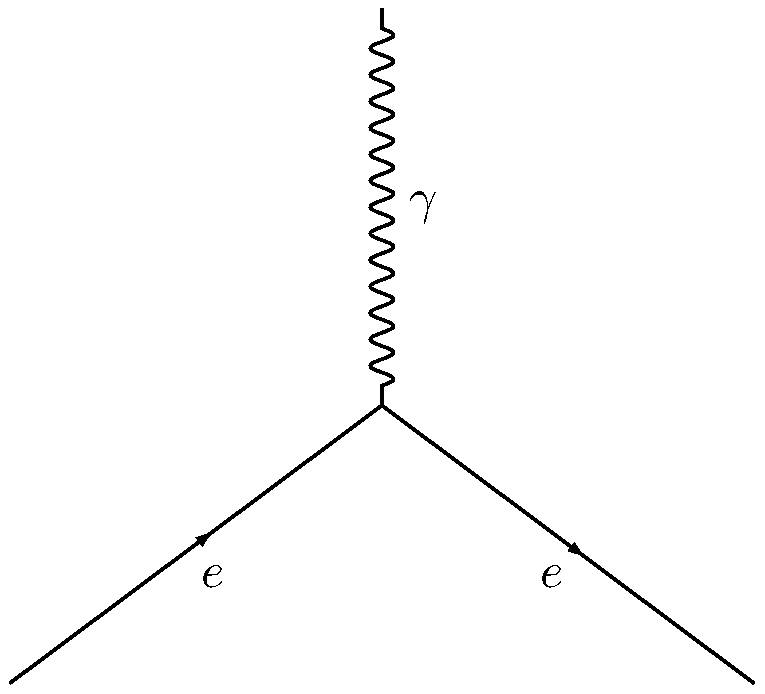
\includegraphics[width=0.25\textwidth]{fig/feynman/forces/qed_vertex.pdf}\label{fig:qed1}}\quad
    \subfloat[]{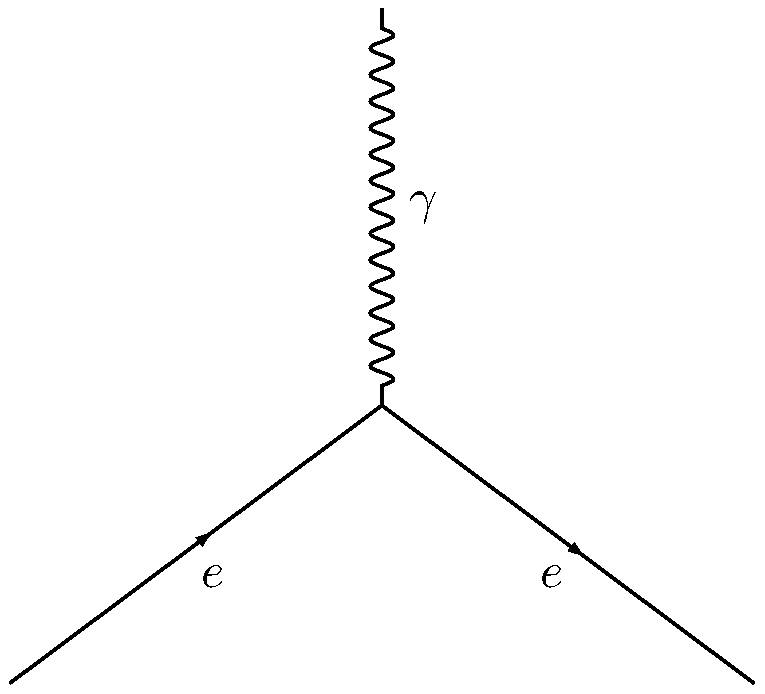
\includegraphics[width=0.25\textwidth]{fig/feynman/forces/qed_vertex.pdf}\label{fig:ewk1}}\quad
    \subfloat[]{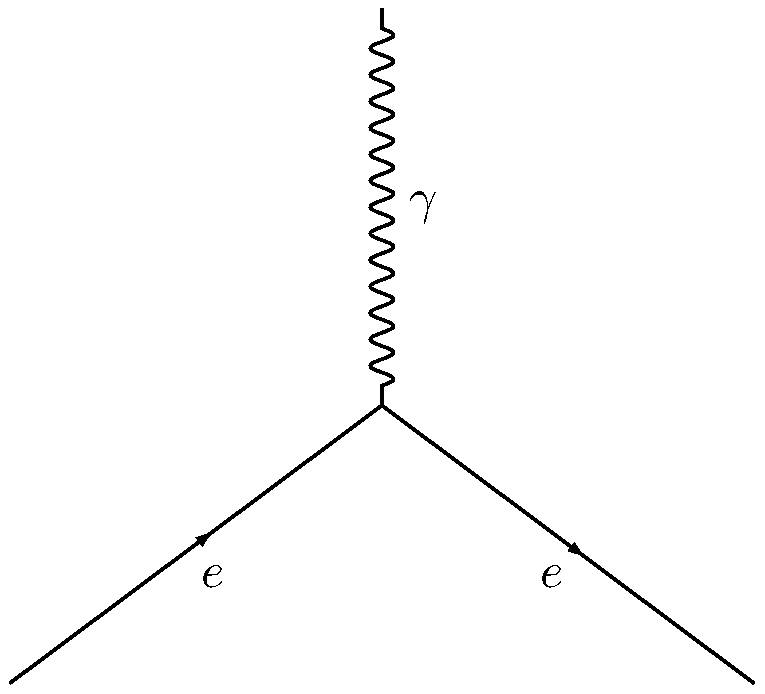
\includegraphics[width=0.25\textwidth]{fig/feynman/forces/qed_vertex.pdf}\label{fig:ewk2}}\\
    \subfloat[]{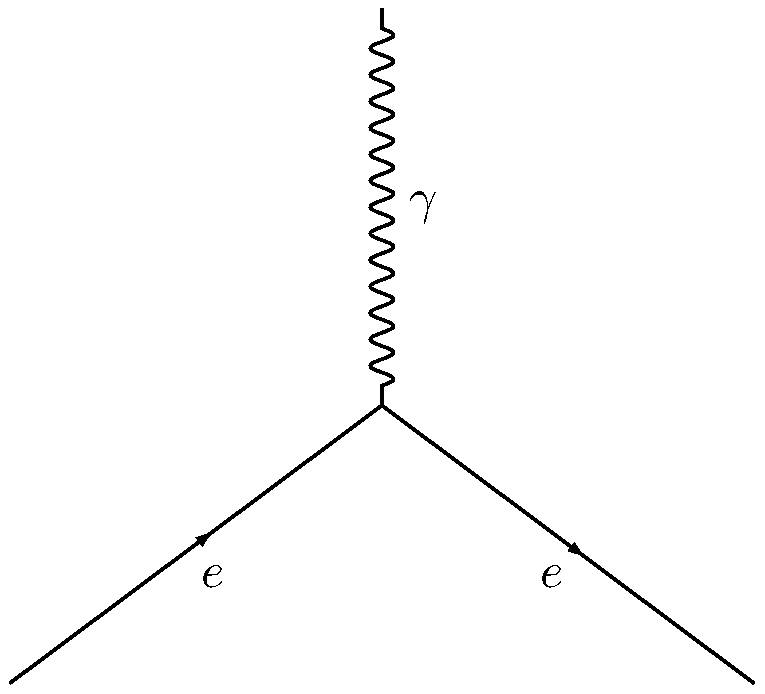
\includegraphics[width=0.25\textwidth]{fig/feynman/forces/qed_vertex.pdf}\label{fig:weak}}\quad
    \subfloat[]{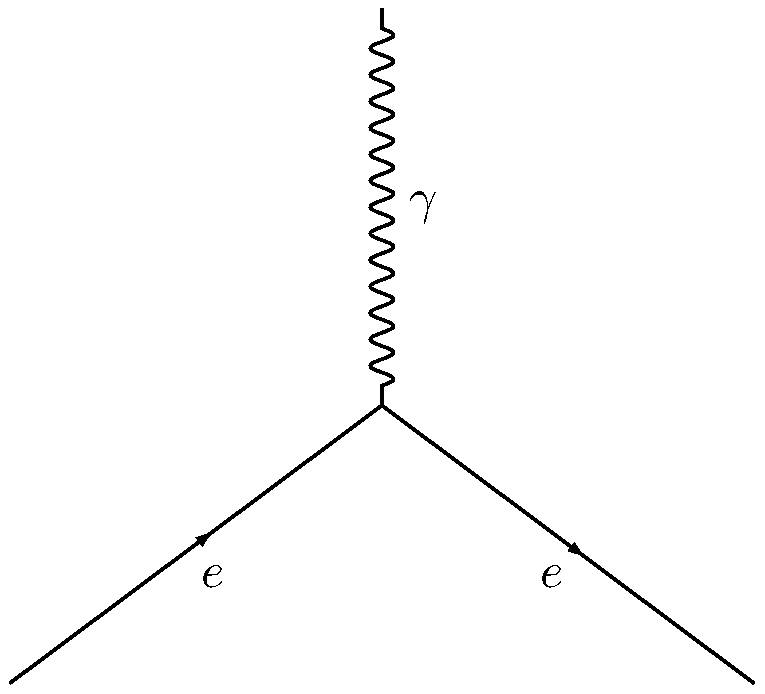
\includegraphics[width=0.25\textwidth]{fig/feynman/forces/qed_vertex.pdf}\label{fig:qcd1}}\quad
    \subfloat[]{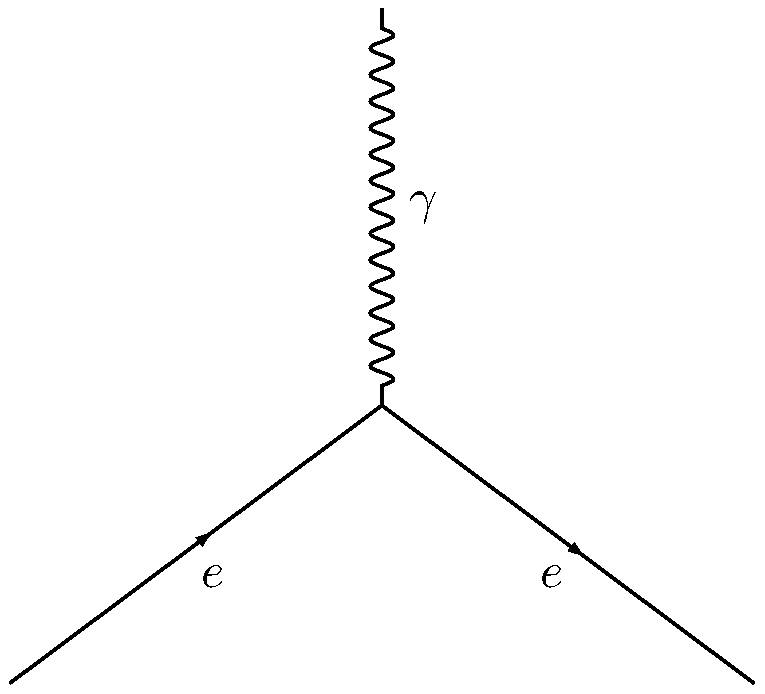
\includegraphics[width=0.25\textwidth]{fig/feynman/forces/qed_vertex.pdf}\label{fig:qcd2}}\\
    \subfloat[]{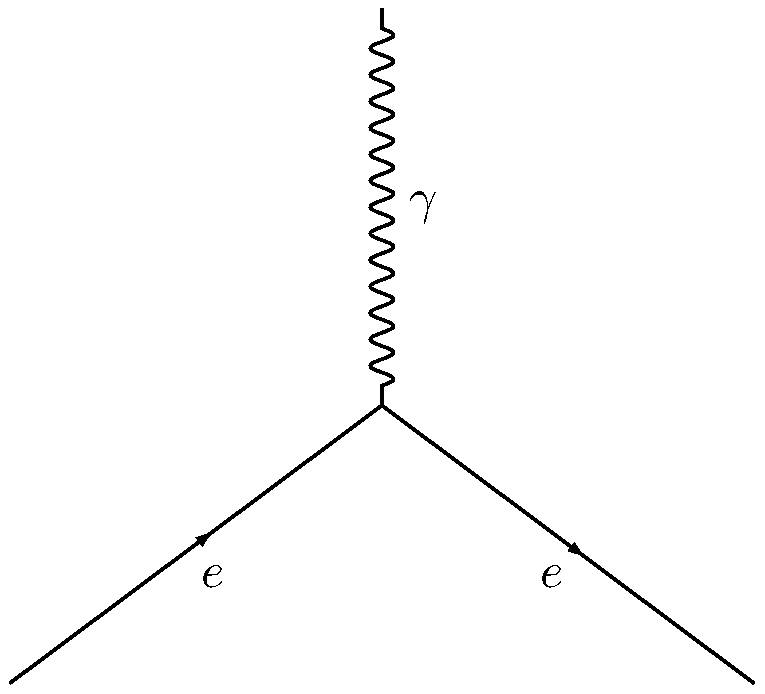
\includegraphics[width=0.25\textwidth]{fig/feynman/forces/qed_vertex.pdf}\label{fig:qcd3}}\quad
    \subfloat[]{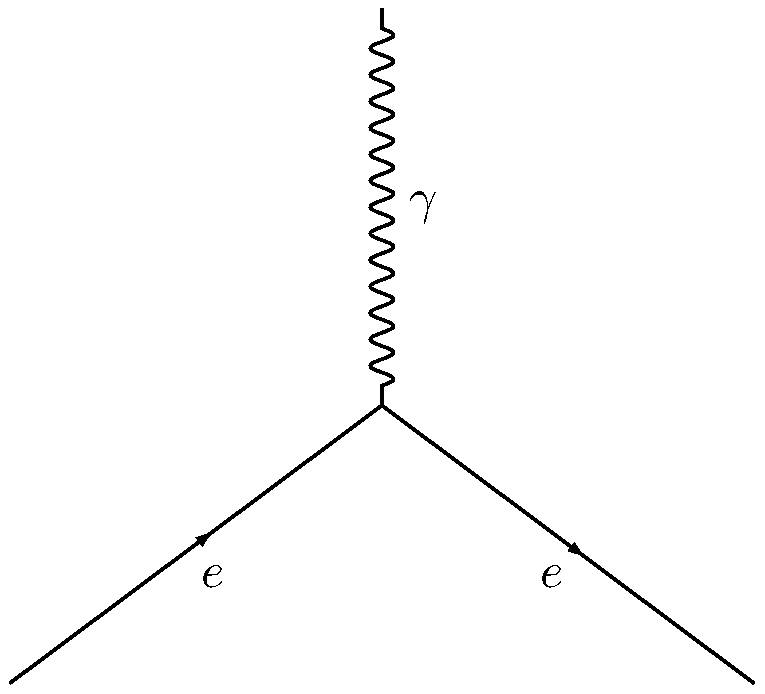
\includegraphics[width=0.25\textwidth]{fig/feynman/forces/qed_vertex.pdf}\label{fig:hig1}}\quad
    \subfloat[]{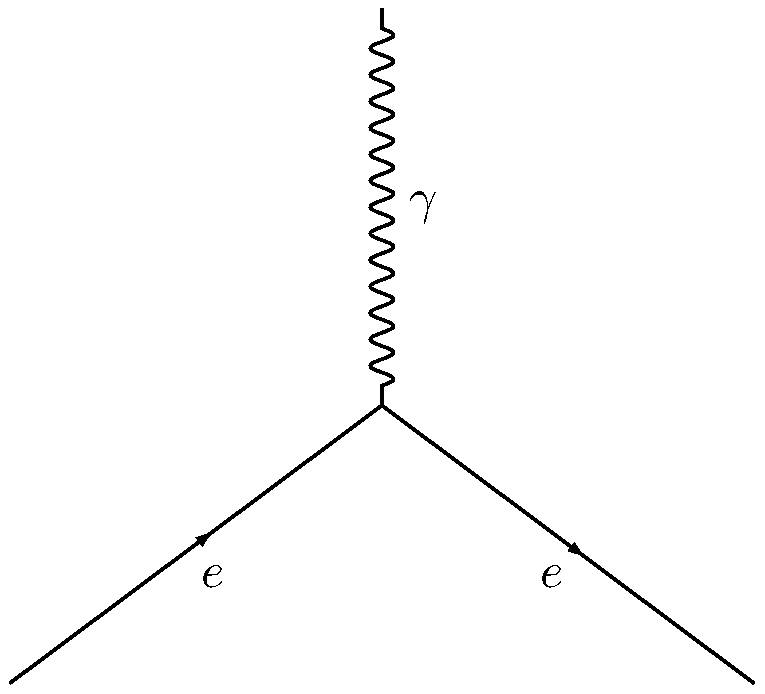
\includegraphics[width=0.25\textwidth]{fig/feynman/forces/qed_vertex.pdf}\label{fig:hig2}}
    \caption{
        The fundamental vertices in the Standard Model. 
        From left to right, top to bottom: 
        (a) electromagnetic; (b), (c) electroweak; (d) weak; (e), (f), (g) strong; (h), (i) Higgs. 
    }
    \label{fig:sm_vertices}
\end{figure}

\subsection{Cross sections}
In order to make the actual mechanics of the Standard Model more clear, consider two electrons barrelling towards each other with some velocity. 
The electrons can, for now, be visualized as two spheres with the same electric charge. 
Finally, the electrons glance off each other and fly off to infinity at some angle to their original respective trajectories. 
This picture can be represented as a Feynman diagram (Fig.~\ref{fig:ee_scattering}) which is assembled by two EM vertices. 
Time flows from left to right in the Feynman diagrams depicted in this document, showing the two electrons entering, then the exchange of a photon, then the two electrons leaving. 
A reasonable question one could ask is ``what is the probability of this collision occuring?''
While this question is entirely quantum mechanical at the scale of electrons, the classical picture of two colliding objects is still useful\footnotemark{}, where this question is answered by computing the cross-sectional area presented to either object. 
\footnote{In fact, the answer to this question is expressed in the units of ``barns,'' literally as in ``hitting the broad side of a barn,'' coined by during World War II.}
Indeed, one of the most important features of QFT is the ability to compute the effective ``cross-section'' for scattering two electrons off of each other, as in this case, or any other interactions between particles. 
Feynman diagrams beautifully encode the complex mathematics at work here according to the ``Feynman Rules.'' 
Along with the momenta of the incoming and outgoing particles, each line and every vertex (where three lines meet) represent a term in the calculation. 
While, again, the mathematical details are beyond the scope of this document, it is important to realize that the Feynman diagram can be directly used to calculate the cross-section ($\sigma$):
\begin{equation}
    \sigma = \langle|\mathcal{M}|^2\rangle = \frac{2g_e^4}{(p_1 \cdot p_3)^2(p_1 \cdot p_4)^2[(p_1 \cdot p_2)^4 + (p_1 \cdot p_3)^4 + (p_1 \cdot p_4)^4]}
\end{equation}
where $p_1$ and $p_2$ are the four-momenta of the incoming electrons, $p_3, p_4$ are the four-momenta of the outgoing electrons, and $g_e$ is the EM coupling constant. 
This exercise, and the compact answer above, serves to demonstrate the sheer complexity of QFT calculations. 
Many details were left out beyond the computation itself (which is already a glaring omission), including details surrounding the spin of the electron, the definition of spin, the defition of four-momentum (and special relativity), and so on. 
These details, and much more, can be found in the illustrious textbook from which the above was borrowed~\cite{Griffiths}. 
Moreover, this feature of QFT---the ability to compute cross-sections---is absolutely vital because it offers a way of testing the theory with observation: compute the probability that the event is expected to occur, then try to reproduce that event many times in the lab and see how many times it really happens. 

\begin{figure}[htb]
    \centering
    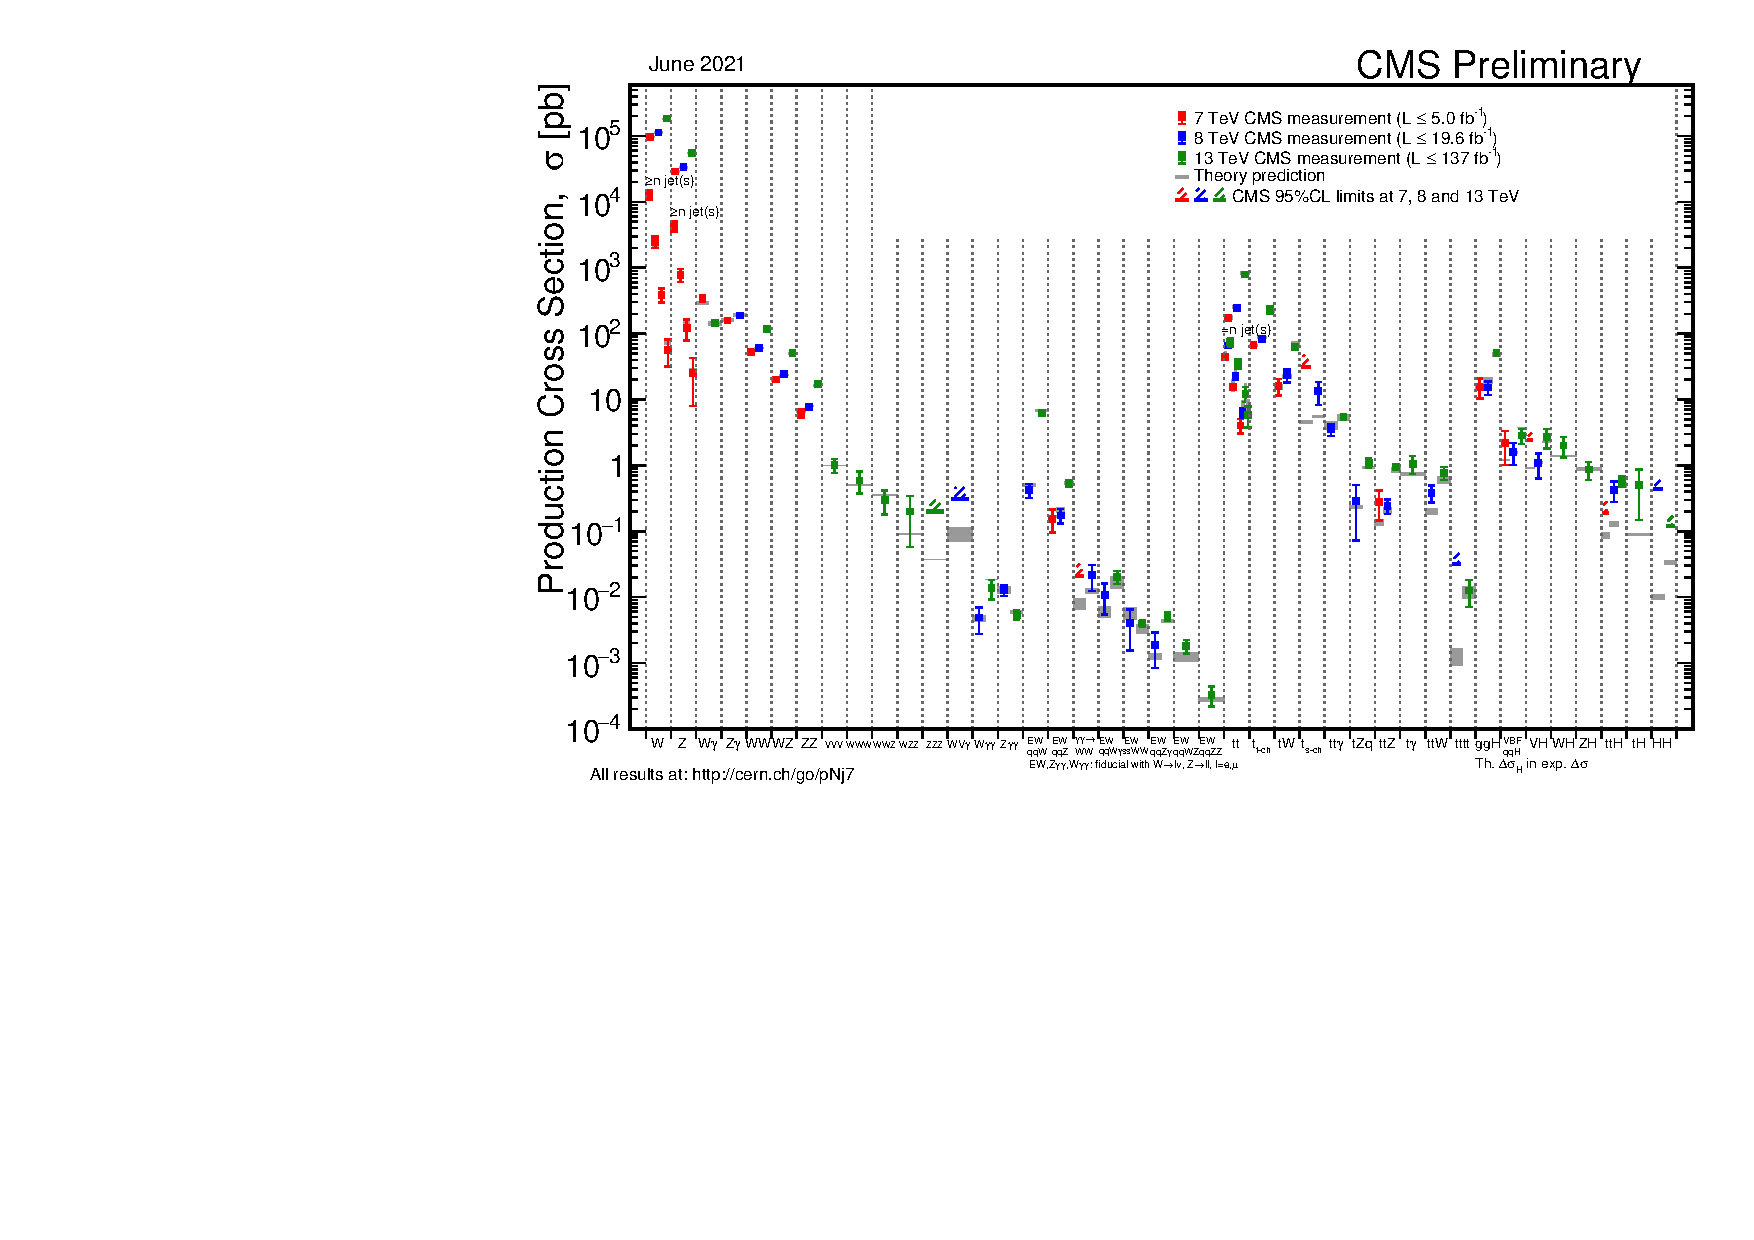
\includegraphics[width=0.8\textwidth]{fig/cms/cms_xsecs_2021.pdf}
    \caption{
        The totality of the cross section measurements performed with data from the CMS Experiment compared to the Standard Model predictions. 
        Precise agreement with the Standard Model can be seen across several orders of magnitude, representing the triumph of the model across decades of experimental scrutiny.
    }
    \label{fig:cms_xsecs}
\end{figure}

% Talk about xsec measurements, how well SM has done, ...
The validity of any model is a precarious condition: the model must exactly describe reality, else it is not a realization of the truth, but rather only approximately---or worse, accidentally---correct. 

\begin{figure}[htb]
    \centering
    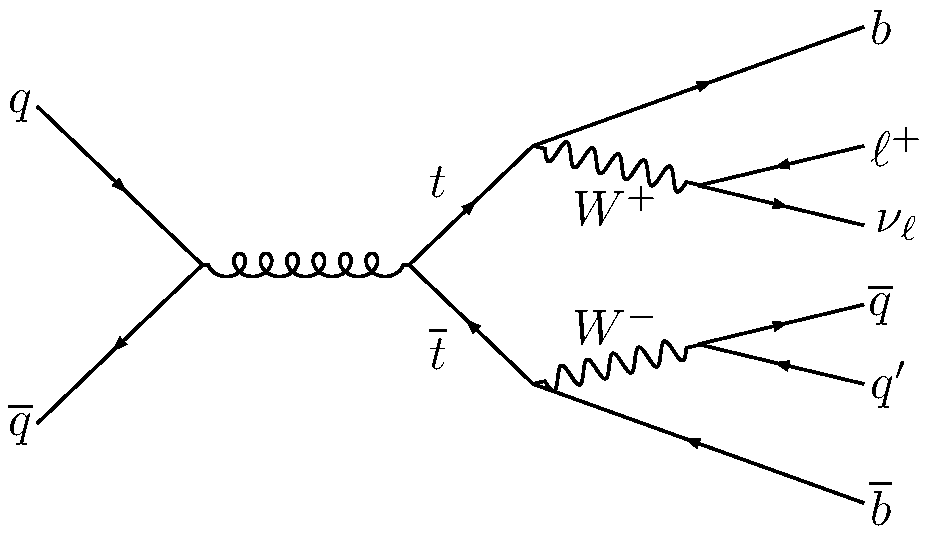
\includegraphics[width=0.8\textwidth]{fig/feynman/ttbar/ttbar_onelep.pdf} % FIXME: missing!!
    \caption{
        Feynman diagram for electron-electron scattering. 
    }
    \label{fig:ee_scattering}
\end{figure}

\subsection{The Higgs boson}
% Give basic overview
%    - wtf is it???
%    - 10-year anniversary Nature papers have a good summary
% From P5:
% The Higgs boson is an extraordinary and unique particle that is connected to the most puzzling questions of particle physics, 
% including the origin of flavor, the matter-antimatter asymmetry, dark matter and dark energy, and inflation. The Higgs boson 
% differs from other particles in that it is “frozen” in the universe. And once frozen, it is called the Higgs field because it 
% permeates the universe. The field disturbs and slows down the motion of every elementary particle. The Higgs boson slows electrons 
% in atoms so that they stay within the atom instead of flying off into space. Without the Higgs boson, or field, every electron 
%
% The Higgs boson is the only known fundamental particle that has no spin angular momentum, which permits it to have unique behavior: 
% it can interact with all known matter particles and give them mass, depending on the strength of the interaction. The Higgs boson 
% also provides a novel and distinct gateway to as yet unknown particles, such as dark matter.
%
% Find sources! Otherwise, this is great
% in every atom would move at the speed of light and everything, including us, would evaporate in a nanosecond.
\section{Open questions}\label{sec:open_questions}
% Higgs sector:
%    - naturalness?
%    - other higgses?? Gell-Mann said something like "it would be weird if 
%      there was only one Higgs boson" in 2012 CERN interview
%    - other problems... I guess introduce problem of not yet measuring 
%      higgs couplings well
% More generic:
%    - dark matter
